\section{Псевдо-значения}

Другой способ думать о складном ноже --- это псевдо-значения
\begin{equation}\label{eq11.14}
    \widetilde{\theta}_{i} = n\hat{\theta} - (n-1)\hat{\theta}_{(i)}.
\end{equation}
Обратите внимание, что в частном случае $\hat{\theta} = \Bar{x}$, мы имеем $\widetilde{\theta}_{i} = x_{i}$, $i$-е значение данных. Кроме того, для любой $\hat{\theta}$ формула для $\widehat{\text{se}}_{\text{jack}}$ может быть выражена как
\begin{equation}\label{eq11.15}
    \widehat{\text{se}}_{\text{jack}} = \left\{\sum\limits_{1}^{n}\left(\tilde{\theta}_{i} - \tilde{\theta}\right)^2/\{(n-1)n\}\right\}^{1/2},
\end{equation}
где $\Tilde{\theta} = \sum\tilde{\theta}_{i}/n$. Это похоже на оценку стандартной ошибки среднего для <<данных>> $\tilde{\theta}_{i},\; i = 1, 2, \dots, n$. Идея, лежащая в основе \ref{eq11.14}, состоит в том, что псевдо-значения должны действовать так, как если бы они были $n$ независимыми значениями.

Что произойдет, если мы попытаемся продолжить эту идею и использовать псевдо-значения для построения доверительного интервала? Один из разумных подходов --- сформировать интервал
\begin{equation}\label{eq11.16}
    \widetilde{\theta} \pm t_{n-1}^{(1-\alpha)}\widehat{\text{se}}_{\text{jack}},
\end{equation}

\noindent
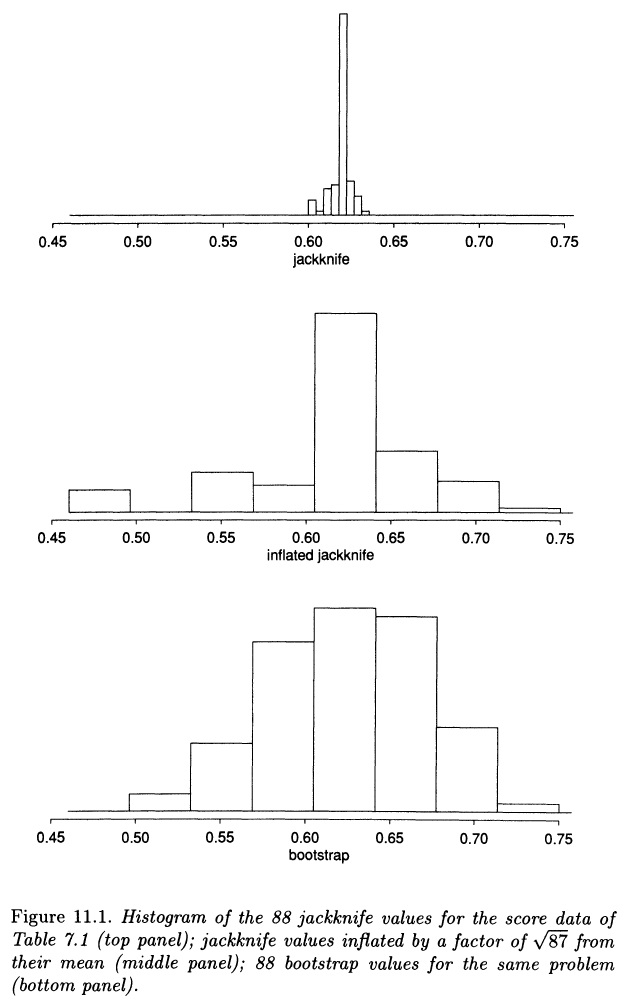
\includegraphics[width=\linewidth]{11/f11.1.jpg}
\newline

\noindentгде $t_{n-1}^{(1-\alpha)}$ --- $(1-\alpha)$-й процентиль распределения $t$ c $n-1$ степеням свободы. Оказывается, этот интервал работает не очень хорошо: в частности, он ненамного лучше, чем более грубые интервалы, основанные на теории о нормальном распределении. Для построения доверительного интервала необходимы более совершенные подходы, как описано в главах 12–14. Хотя псевдо-значения интригуют, неясно, являются ли они хороший способ думать о складном ноже. Мы не будем здесь их рассматривать.